
\begin{figure}[h]
\centering
\tikzset{every picture/.style={line width=0.75pt}} %set default line width to 0.75pt        

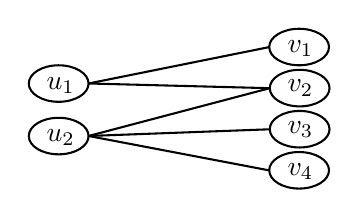
\begin{tikzpicture}[x=0.75pt,y=0.75pt,yscale=-.55,xscale=.9]
%uncomment if require: \path (0,310); %set diagram left start at 0, and has height of 310

%Shape: Circle [id:dp705325080636104] 
\draw   (237.14,68.73) .. controls (237.17,77.56) and (230.04,84.76) .. (221.2,84.79) .. controls (212.37,84.83) and (205.17,77.7) .. (205.14,68.86) .. controls (205.1,60.02) and (212.23,52.83) .. (221.07,52.79) .. controls (229.91,52.76) and (237.1,59.89) .. (237.14,68.73) -- cycle ;
%Shape: Circle [id:dp9045264439682683] 
\draw   (236.86,32.73) .. controls (236.9,41.56) and (229.76,48.76) .. (220.93,48.79) .. controls (212.09,48.83) and (204.9,41.7) .. (204.86,32.86) .. controls (204.82,24.03) and (211.96,16.83) .. (220.79,16.8) .. controls (229.63,16.76) and (236.82,23.89) .. (236.86,32.73) -- cycle ;
%Shape: Circle [id:dp7330157492007956] 
\draw   (108.14,64.73) .. controls (108.17,73.56) and (101.04,80.76) .. (92.2,80.79) .. controls (83.37,80.83) and (76.17,73.7) .. (76.14,64.86) .. controls (76.1,56.02) and (83.23,48.83) .. (92.07,48.79) .. controls (100.91,48.76) and (108.1,55.89) .. (108.14,64.73) -- cycle ;
%Shape: Circle [id:dp6777718508352495] 
\draw   (236.86,140.73) .. controls (236.9,149.56) and (229.76,156.76) .. (220.93,156.79) .. controls (212.09,156.83) and (204.9,149.7) .. (204.86,140.86) .. controls (204.82,132.03) and (211.96,124.83) .. (220.79,124.8) .. controls (229.63,124.76) and (236.82,131.89) .. (236.86,140.73) -- cycle ;
%Shape: Circle [id:dp5798086220020264] 
\draw   (237.14,104.73) .. controls (237.17,113.56) and (230.04,120.76) .. (221.2,120.79) .. controls (212.37,120.83) and (205.17,113.7) .. (205.14,104.86) .. controls (205.1,96.02) and (212.23,88.83) .. (221.07,88.79) .. controls (229.91,88.76) and (237.1,95.89) .. (237.14,104.73) -- cycle ;
%Shape: Circle [id:dp6665288116424322] 
\draw   (108.14,110.73) .. controls (108.17,119.56) and (101.04,126.76) .. (92.2,126.79) .. controls (83.37,126.83) and (76.17,119.7) .. (76.14,110.86) .. controls (76.1,102.02) and (83.23,94.83) .. (92.07,94.79) .. controls (100.91,94.76) and (108.1,101.89) .. (108.14,110.73) -- cycle ;
%Straight Lines [id:da6695348841913797] 
\draw    (108.14,64.73) -- (204.86,32.86) ;
%Straight Lines [id:da13011748270531487] 
\draw    (108.14,64.73) -- (205.14,68.86) ;
%Straight Lines [id:da41568081525275913] 
\draw    (108.14,110.73) -- (205.14,68.86) ;
%Straight Lines [id:da387934327631003] 
\draw    (108.14,110.73) -- (205.14,104.86) ;
%Straight Lines [id:da9311827336887017] 
\draw    (108.14,110.73) -- (204.86,140.86) ;

% Text Node
\draw (213,59) node [anchor=north west][inner sep=0.75pt]   [align=left] {{$v_2$}};
% Text Node
\draw (213,24) node [anchor=north west][inner sep=0.75pt]   [align=left] {{$v_1$}};
% Text Node
\draw (213,132) node [anchor=north west][inner sep=0.75pt]   [align=left] {{$v_4$}};
% Text Node
\draw (213,95) node [anchor=north west][inner sep=0.75pt]   [align=left] {{$v_3$}};

% Text Node
\draw (84,57) node [anchor=north west][inner sep=0.75pt]   [align=left] {{$u_1$}};
% Text Node
\draw (84,102) node [anchor=north west][inner sep=0.75pt]   [align=left] {{$u_2$}};

\end{tikzpicture}
\caption{Depending on $\prob\in\{1/4,.5,1\}$ the instance is $1/2$-oversupplied, balanced, or $2$-undersupplied.}\label{fig:example_imbalance}
\end{figure}